This section presents the main results of the one hundred and twenty experiments performed as defined in Section \ref{subsec:experimental_design}. The experiments are grouped into subsections according to the measured operation, i.e., read or write. Each subsection presents histograms and tables to visualize the results using both metrics, i.e., latency and throughput. Latency is expressed in seconds, and throughput is represented in rows/second.

Results are reported using the log scale for clarity, as results differing from more than one significant figure are not clearly visible using a linear scale in a histogram representation. Additionally, for each measurement, a 95\% confidence interval was calculated using the bootstrapping technique mentioned in Section \ref{subsec:reliability_validity}. Nonetheless, this interval was not reported in the histograms in this section, as it would be hardly readable. This is because all results are out of each other's 95\% confidence interval. This data is reported in the Appendix \ref{appx:res_write} and \ref{appx:res_read} with a histogram and a table for each experiment expressed in both metrics.

Of the two metrics defined in RQ2, only latency was measured during the experiments, while throughput was calculated with the formula present in Section ~\ref{subsec:eval_process}. Latency and throughput are inversely correlated by a constant factor since all experiments were performed with fixed-size tables. This relationship means that if latency is halved, throughput doubles, if latency quarters, throughput quadruples. Since results are reported according to both metrics, this creates an information redundancy. Trends will be described using latency to avoid repetition in this section. Throughput trends will be described if they reflect a significant behavior different from the latency trends.

\subsection{Write experiments}

\begin{figure}
    \centering
    \begin{minipage}[b]{\textwidth}
        \centering
        \captionof{table}[Write experiments results expressed as latency]{Write experiment results expressed as latency. Experiments performed with more than one \glstext{CPU} core are expressed as latency percentage decrease compared to the one \glstext{CPU} core experiment.}
        \label{tbl:res_write_time_cpu_perc}
        \begin{tabular}{c r S[table-format=4.5] S[table-format=2.2] S[table-format=2.2] S[table-format=2.2]} 
            \toprule
            Pipeline\Tstrut\Bstrut & \thead{Number\\ of rows} & {\thead{1 CPU core latency \\ (seconds)}} & {\thead{2 CPU cores\\ (\% decrease)}} & {\thead{4 CPU cores\\ (\% decrease)}} & {\thead{8 CPU cores\\ (\% decrease)}} \\
            \midrule
            \multirow{5}{4em}{delta-rs\\ HopsFS} & 10K & 1.25088 & -0.92 & 2.75 & -9.33\\ 
            & 100K & 1.36828 & 4.40 & 2.34 & 5.54\\ 
            & 1M &   9.38152 & 9.23 & 10.32 & 11.52\\
            & 6M &   19.75469 & 17.54 & 17.87 & 20.33\\
            & 60M &  177.30707 & 24.39 & 30.01 & 31.22\\
            \midrule
            \multirow{5}{4em}{delta-rs\\ LocalFS} & 10K & 0.03957 & -21.88 & -15.53 & -11.25\\ 
            & 100K & 0.15240 & 10.01 & 13.54 & 10.45\\ 
            & 1M &   8.42252 & 14.69 & 14.68 & 14.17\\
            & 6M &   17.90634 & 14.74 & 18.71 & 20.24\\
            & 60M &  172.34552 & 24.67 & 29.57 & 30.38\\
            \midrule
            \multirow{5}{4em}{Legacy} & 10K & 50.22767 & -0.99 & -2.10 & -1.99\\ 
            & 100K & 59.56187 & -0.38 & 0.06 & -1.20\\ 
            & 1M &   112.19048 & 3.23 & 3.01 & 2.50\\
            & 6M &   511.81693 & 7.51 & 5.83 & 7.01\\
            & 60M &  2715.77285 & 13.81 & 13.61 & 14.39\\
            \bottomrule
        \end{tabular}
    \end{minipage}
    \begin{minipage}[b]{\textwidth}
        \centering
        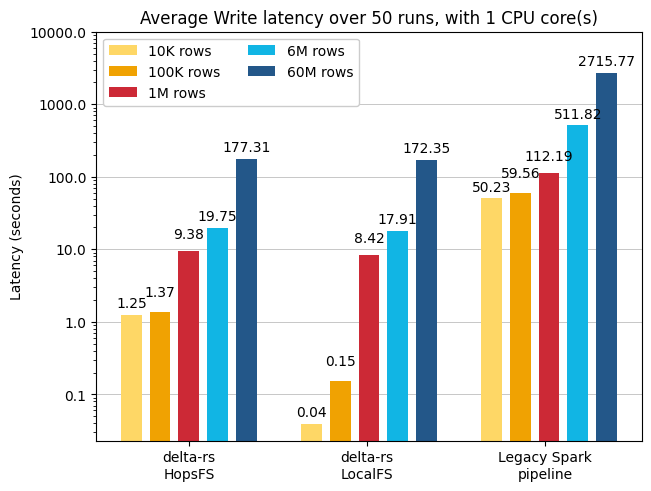
\includegraphics[width=\textwidth]{figures/5-results/write/write_time_1_core.png}
        \caption[Histogram of the write experiment - Latency - 1 CPU core]{Histogram in log-scale of the write experiment results expressed as latency. The experiment was performed with one \glstext{CPU} core.}
        \label{fig:res_write_time}
    \end{minipage}
\end{figure}

\begin{figure}
    \centering
    \begin{minipage}[b]{\textwidth}
        \captionof{table}[Write experiments results expressed as throughput]{Write experiment results expressed as throughput. Experiments performed with more than one \glstext{CPU} core are expressed as throughput percentage increase compared to the one \glstext{CPU} core experiment.}
        \label{tbl:res_write_throughput_cpu_perc}
        \begin{tabular}{c r S[table-format=4.5] S[table-format=2.2] S[table-format=2.2] S[table-format=2.2]}
            \toprule
            Pipeline\Tstrut\Bstrut & {\thead{Number\\ of rows}} & {\thead{1 CPU core throughput \\ (k rows/second)}} & {\thead{2 CPU cores\\ (\% increase)}} & {\thead{4 CPU cores\\ (\% increase)}} & {\thead{8 CPU cores\\ (\% increase)}} \\
            \midrule
            \multirow{5}{4em}{delta-rs\\ HopsFS} & 10K & 7.99436 & -0.91 & 2.83 & -8.53\\ 
            & 100K & 73.08438 & 4.60 & 2.40 & 5.87\\ 
            & 1M &   106.59242 & 10.17 & 11.51 & 13.01\\
            & 6M &   303.72533 & 21.27 & 21.76 & 25.52\\
            & 60M &  338.39598 & 32.26 & 42.87 & 45.39\\
            \midrule
            \multirow{5}{4em}{delta-rs\\ LocalFS} & 10K & 252.68238 & -17.95 & -13.44 & -10.12\\ 
            & 100K & 656.15739 & 11.13 & 15.66 & 11.67\\ 
            & 1M &   118.72919 & 17.22 & 17.21 & 16.51\\
            & 6M &   335.07675 & 17.29 & 23.02 & 25.38\\
            & 60M &  348.13784 & 32.76 & 41.99 & 43.65\\
            \midrule
            \multirow{5}{4em}{Legacy} & 10K & 0.19909 & -0.98 & -2.06 & -1.95\\ 
            & 100K & 1.67892 & -0.38 & 0.06 & -1.19\\ 
            & 1M &   8.91341 & 3.34 & 3.10 & 2.57\\
            & 6M &   11.72294 & 8.12 & 6.19 & 7.54\\
            & 60M &  22.09315 & 16.02 & 15.76 & 16.81\\
            \bottomrule
        \end{tabular}
    \end{minipage}
    \begin{minipage}[b]{\textwidth}
        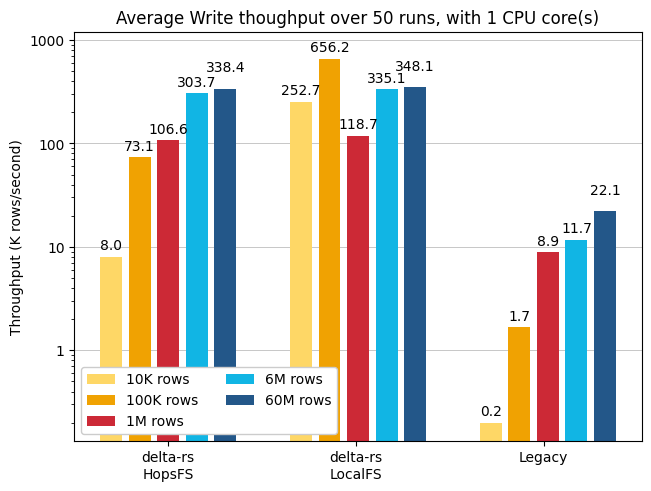
\includegraphics[width=\textwidth]{figures/5-results/write/write_throughput_1_core.png}
        \caption[Histogram of the write experiment - Throughput - 1 CPU core]{Histogram in log-scale of the write experiment results expressed as throughput. The experiment was performed with one \glstext{CPU} core.}
        \label{fig:res_write_throughput}
    \end{minipage}
\end{figure}

Figures~\ref{fig:res_write_time} and \ref{fig:res_write_throughput}, and Tables~\ref{tbl:res_write_time_cpu_perc} and \ref{tbl:res_write_throughput_cpu_perc} report the results of the write experiments performed. The results are expressed in latency in Figure~\ref{fig:res_write_time} and Table~\ref{tbl:res_write_time_cpu_perc}, and expressed in throughput in Figure~\ref{fig:res_write_throughput} and Table~\ref{tbl:res_write_throughput_cpu_perc}. The experiments were performed on the three systems defined in Section~\ref{subsec:experimental_design}. The five tables of different sizes being written were defined in Section~\ref{subsec:data}.

Both histograms, i.e., Figures~\ref{fig:res_write_time} and \ref{fig:res_write_throughput}, report the results of the experiment performed with one \gls{CPU} core. On the other hand, the Tables~\ref{tbl:res_write_time_cpu_perc} and \ref{tbl:res_write_throughput_cpu_perc} on top of reporting the results of the one \gls{CPU} core experiment also present a calculated percentage of improvement (decrease in the case of latency, increase in the case of throughput) of the metric as the \gls{CPU} cores increase.

\subsubsection*{delta-rs on \glsentryshort{HopsFS} vs. delta-rs on \glsentryshort{LocalFS}}

The latency measured using the delta-rs on \gls{LocalFS} pipeline is around ten times lower than the latency measured using the delta-rs on \gls{HopsFS} pipeline for small tables, i.e., 10K and 100K rows. On the other hand, the latency in the two pipelines has the same significant figure in experiments performed with larger tables, i.e., 1M, 10M, 6M, and 60M rows. Overall, the latency measured in the delta-rs on \gls{LocalFS} pipeline remains lower in absolute terms than the latency measured using the delta-rs on \gls{HopsFS} pipeline in all experiments.

\subsubsection*{delta-rs on \glsentryshort{HopsFS} vs. Legacy pipeline}

The latency measured using the delta-rs on \gls{HopsFS} pipeline results more than ten times lower than the latency measured using the Legacy pipeline in all experiments. This trend is more prominent for smaller tables (10K and 100K rows) where latency measured using the delta-rs on \gls{HopsFS} pipeline is forty times lower than the latency measured using the Legacy pipeline. The tendency is less marked for larger tables (6M and 60M rows) where latency measured using the delta-rs on \gls{HopsFS} pipeline is around twenty times lower than the latency measured using the Legacy pipeline.

\subsubsection*{Change of performance as the \glsentryshort{CPU} cores increase}

During experiments with more \gls{CPU} cores, in delta-rs based pipelines (writing on \gls{HopsFS} or \gls{LocalFS}) the latency during write operation decreases by a considerable amount: 20-30\%, only when writing larger tables (6M and 60M rows), while it decreases by a lower margin: 5-10\% on smaller tables (100K and 1M rows), even slightly increasing on the smallest table (10K rows). It should be noted that latency decreases as described in the two \gls{CPU} cores experiments, remaining on similar improvements even with more \gls{CPU} cores.

Considering the Legacy pipeline, experiments with more \gls{CPU} cores did not decrease the latency by more than 7\% except for the largest table (60M rows). This table benefitted from a latency decrease of around 14\%. The smallest tables (10K and 100K) reported slight increases in the measured latency.

\subsection{Read experiments}

\begin{figure}
    \centering
    \begin{minipage}[b]{\textwidth}
        \captionof{table}[Read experiments results expressed as latency]{Read experiment results expressed as latency. Experiments performed with more than one \glstext{CPU} core are expressed as latency percentage decrease compared to the one \glstext{CPU} core experiment.}
        \label{tbl:res_read_time_cpu_perc}
        \begin{tabular}{c r S[table-format=4.5] S[table-format=2.2] S[table-format=2.2] S[table-format=2.2]} 
            \toprule
            Pipeline\Tstrut\Bstrut & {\thead{Number\\ of rows}} & {\thead{1 CPU core latency \\ (seconds)}} & {\thead{2 CPU cores\\ (\% decrease)}} & {\thead{4 CPU cores\\ (\% decrease)}} & {\thead{8 CPU cores\\ (\% decrease)}} \\
            \midrule
            \multirow{5}{4em}{delta-rs\\ HopsFS} & 10K & 0.05342 & 22.65 & 18.84 & 18.95\\ 
            & 100K & 0.05757 & 1.15 & 3.76 & 5.19\\ 
            & 1M & 0.53855 & 56.53 & 65.00 & 67.71\\
            & 6M & 1.94899 & 53.40 & 72.74 & 74.48\\
            & 60M & 22.98065 & 50.34 & 75.72 & 87.20\\
            \midrule
            \multirow{5}{4em}{delta-rs\\ LocalFS} & 10K & 0.00419 & 31.48 & 35.91 & 29.66\\ 
            & 100K & 0.02696 & 51.54 & 65.76 & 64.84\\ 
            & 1M &   0.42009 & 52.45 & 78.64 & 89.75\\
            & 6M &   1.68223 & 55.56 & 77.99 & 89.57\\
            & 60M &  19.56547 & 51.72 & 75.41 & 88.32\\
            \midrule
            \multirow{5}{4em}{Legacy} & 10K & 0.63159 & 1.06 & -0.67 & 0.67\\ 
            & 100K & 2.65010 & -0.50 & 0.39 & -0.46\\ 
            & 1M &   8.59636 & -0.24 & -1.81 & 2.89\\
            & 6M &   33.52964 & 0.46 & 0.23 & 0.30\\
            & 60M &  33.69772 & 0.16 & 0.13 & 1.64\\
            \bottomrule
        \end{tabular}
    \end{minipage}
    \begin{minipage}[b]{\textwidth}
        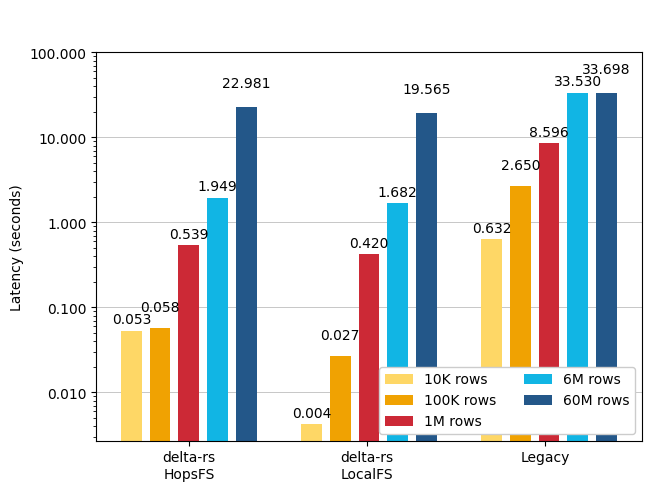
\includegraphics[width=\textwidth]{figures/5-results/read/read_time_1_core.png}
        \caption[Histogram of the read experiment - Latency - 1 CPU core]{Histogram in log-scale of the read experiment results expressed as latency. The experiment was performed with one \glstext{CPU} core.}
        \label{fig:res_read_time}
    \end{minipage}
\end{figure}

\begin{figure}
    \centering
    \begin{minipage}[b]{\textwidth}
        \captionof{table}[Read experiments results expressed as throughput]{Read experiment results expressed as throughput. Experiments performed with more than one \glstext{CPU} core are expressed as throughput percentage increase compared to the one \glstext{CPU} core experiment.}
        \label{tbl:res_read_throughput_cpu_perc}
        \begin{tabular}{c r S[table-format=4.5] S[table-format=2.2] S[table-format=2.2] S[table-format=2.2]}
            \toprule
            Pipeline\Tstrut\Bstrut & {\thead{Number\\ of rows}} & {\thead{1 CPU core throughput \\ (k rows/second)}} & {\thead{2 CPU cores\\ (\% increase)}} & {\thead{4 CPU cores\\ (\% increase)}} & {\thead{8 CPU cores\\ (\% increase)}} \\
            \midrule
            \multirow{5}{4em}{delta-rs\\ HopsFS} & 10K & 187.16853 & 29.28 & 23.21 & 23.38\\ 
            & 100K & 1736.90799 & 1.17 & 3.90 & 5.48\\ 
            & 1M &   1856.83167 & 130.02 & 185.74 & 209.69\\
            & 6M &   3078.51299 & 114.57 & 266.87 & 291.92\\
            & 60M &  2610.89146 & 101.35 & 311.83 & 681.03\\
            \midrule
            \multirow{5}{4em}{delta-rs\\ LocalFS} & 10K & 2384.58699 & 45.94 & 56.04 & 42.18\\ 
            & 100K & 3708.25787 & 106.37 & 192.07 & 184.38\\ 
            & 1M &   2380.40381 & 110.28 & 368.24 & 875.15\\
            & 6M &   3566.67454 & 125.01 & 354.40 & 858.64\\
            & 60M &  3066.62644 & 107.11 & 306.75 & 756.07\\
            \midrule
            \multirow{5}{4em}{Legacy} & 10K & 15.83285 & 1.07 & -0.67 & 0.67\\ 
            & 100K & 37.73432 & -0.50 & 0.39 & -0.45\\ 
            & 1M &   116.32820 & -0.24 & -1.78 & 2.98\\
            & 6M &   178.94612 & 0.46 & 0.23 & 0.30\\
            & 60M &  1780.53563 & 0.16 & 0.13 & 1.67\\
            \bottomrule
        \end{tabular}
    \end{minipage}
    \begin{minipage}[b]{\textwidth}
        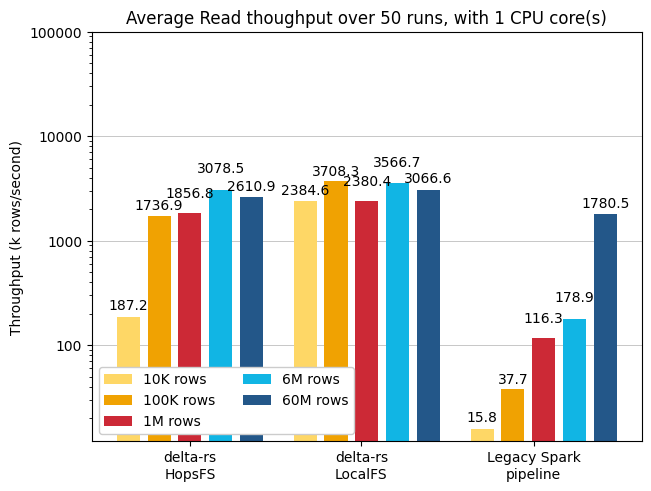
\includegraphics[width=\textwidth]{figures/5-results/read/read_throughput_1_core.png}
        \caption[Histogram of the read experiment - Throughput - 1 CPU core]{Histogram in log-scale of the read experiment results expressed as throughput. The experiment was performed with one \glstext{CPU} core.}
        \label{fig:res_read_throughput}
    \end{minipage}
\end{figure}

Figures~\ref{fig:res_read_time} and \ref{fig:res_read_throughput}, and Tables~\ref{tbl:res_write_time_cpu_perc} and \ref{tbl:res_read_throughput_cpu_perc} report the results of the read experiments performed. The results are expressed in latency in Figure~\ref{fig:res_read_time} and Table~\ref{tbl:res_read_time_cpu_perc}, and expressed in throughput in Figure~\ref{fig:res_read_throughput} and Table~\ref{tbl:res_read_throughput_cpu_perc}. The experiments were performed on the three systems defined in Section~\ref{subsec:experimental_design}. The five tables of different sizes being written were defined in Section~\ref{subsec:data}.

Both histograms, i.e., Figures~\ref{fig:res_read_time} and \ref{fig:res_read_throughput} report the results of the experiment performed with one \gls{CPU} core. On the other hand, the Tables~\ref{tbl:res_read_time_cpu_perc} and \ref{tbl:res_read_throughput_cpu_perc} on top of reporting the results of the one \gls{CPU} core experiment also present a calculated percentage of improvement (decrease in the case of latency, increase in the case of throughput) of the metric as the \gls{CPU} cores increase.

\subsubsection*{delta-rs on \glsentryshort{HopsFS} vs. delta-rs on \glsentryshort{LocalFS}}

The latency measured using the delta-rs on \gls{LocalFS} pipeline is around ten times lower than the latency measured using the delta-rs on \gls{HopsFS} pipeline in the experiment with the smallest table, i.e., 10K rows. On the other hand, the latency in the two pipelines has the same significant figure on experiments performed with larger tables, i.e., 100K, 1M, 10M, 6M, and 60M rows. Overall, the latency measured in the delta-rs on \gls{LocalFS} pipeline remains lower in absolute terms than the latency measured using the delta-rs on \gls{HopsFS} pipeline in all experiments.

\subsubsection*{delta-rs on \glsentryshort{HopsFS} vs. Legacy pipeline}

The latency measured using the delta-rs on \gls{HopsFS} pipeline results from 47\% up to forty times lower than the latency measured using the Legacy pipeline. The largest latency reduction compared to the legacy system (forty times) is obtained with the 100K rows table. In contrast, the smallest decrease in latency between newer and older systems is obtained with the largest table, i.e., 60M rows. For all other tables, the delta-rs on \gls{HopsFS} pipeline has around ten times lower latency than the legacy system.

\subsubsection*{Change of performance as the \glsentryshort{CPU} cores increase}

During experiments with more \gls{CPU} cores, in delta-rs based pipelines (reading on \gls{HopsFS} or \gls{LocalFS}), the latency during read operation decreases by a considerable amount: 50\%, when reading larger tables (1M, 6M and 60M rows), while it decreases by a lower margin: 20-30\% on smaller tables, i.e., 10K and 100K rows. It should be noted that latency decreases in reads with larger tables (1M, 6M, and 60M rows) following an inverse linear relationship with the increase of \gls{CPU} cores: two \gls{CPU} cores, latency halves, four \gls{CPU} cores, latency quarters, eight \gls{CPU} cores, latency is decreased to an eighth. On the other hand, throughput follows a linear relationship with the increase of \gls{CPU} cores.

Considering the Legacy pipeline, experiments with more \gls{CPU} cores did not decrease the latency by more than 2\%. Histograms comparing the three pipelines look radically different in experiments with more \gls{CPU} cores due to how delta-rs scales with the increase of \gls{CPU} cores. They can be accessed in the Appendix \ref{appx:res_write}.

\subsection{Legacy pipeline write latency breakdown}

\begin{figure}
    \centering
    \begin{minipage}[b]{\textwidth}
        \captionof{table}[Writes on legacy pipeline - Time breakdown]{Contributions to the write latency of the upload and materialization steps in the legacy pipeline. Experiments performed with more than one \glstext{CPU} core are expressed as latency percentage decrease compared to the one \glstext{CPU} core experiment.}
        \label{tbl:hudi_virtualiz_breakdown_cpu_perc}
        \begin{tabular}{r S[table-format=4.2] S[table-format=4.2] S[table-format=2.2] S[table-format=2.2] S[table-format=2.2] S[table-format=2.2] S[table-format=2.2] S[table-format=2.2]} 
            \toprule
            \multirow{2}{*}{{\thead{Number\\ of rows}}} & \multicolumn{2}{c}{{\thead{1 CPU core\\ latency (seconds)}}} & \multicolumn{2}{c}{{\thead{2 CPU cores\\ (\% decrease)}}} & \multicolumn{2}{c}{{\thead{4 CPU cores\\ (\% decrease)}}} & \multicolumn{2}{c}{{\thead{8 CPU cores\\ (\% decrease)}}}\\
            & {upl.} & {mat.} & {upl.} & {mat.} & {upl.} & {mat.} & {upl.} & {mat.}\\
            \midrule
            10K &  2.48 & 47.72 & 3.99 & -1.27 & 4.10 & -2.47 & 4.22 & -2.35\\
            100K & 3.66 & 55.90 & 6.37 & -0.78 & 5.55 & -0.27 & 6.25 & -1.69\\
            1M   & 22.59 & 89.57 & 17.52 & -0.39 & 14.89 & -0.01 & 16.51 & -1.05\\
            6M   & 244.61 & 267.24 & 15.83 & -0.10 & 13.46 & -1.15 & 15.10 & -0.38\\
            60M &  2437.78 & 278.05 & 15.33 & 0.39 & 15.15 & 0.16 & 15.94 & 0.82\\
            \bottomrule
        \end{tabular}
    \end{minipage}
    \begin{minipage}[b]{\textwidth}
        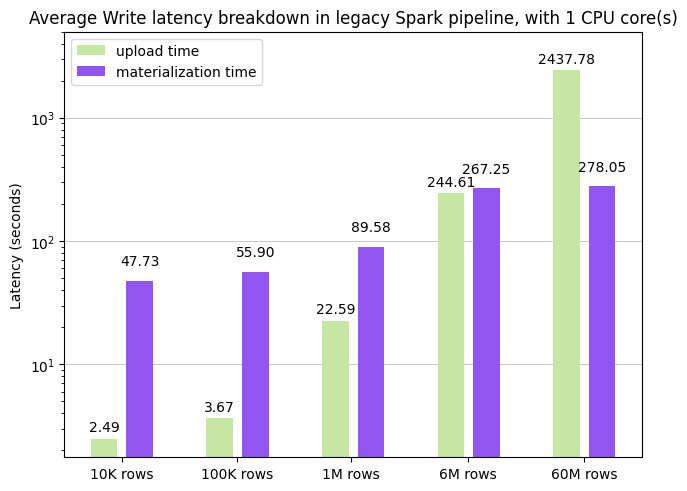
\includegraphics[width=\textwidth]{figures/5-results/hudi_virtualiz_1_core.png}
        \caption[Histogram of the write on legacy pipeline - Time breakdown - 1 core]{Histogram in log-scale displaying the contributions to the write latency of the upload and materialization steps in the legacy pipeline. The experiment was performed with one \glstext{CPU} core.}
        \label{fig:hudi_virtualiz_breakdown}
    \end{minipage}
\end{figure}

Table \ref{tbl:hudi_virtualiz_breakdown_cpu_perc} and Figure \ref{fig:hudi_virtualiz_breakdown} show the write latency breakdown of the Legacy pipeline into upload time and materialization time, the different steps of the Legacy pipeline as explained in Section \ref{subsec:legacy_sys_writing}. The breakdown is proposed for all five tables defined in Section \ref{subsec:data}. Figure \ref{fig:hudi_virtualiz_breakdown} reports the data from the one \gls{CPU} core experiment. In contrast, Table \ref{tbl:hudi_virtualiz_breakdown_cpu_perc} reports both the one \gls{CPU} core experiment data and also a calculated percentage of improvement, i.e., decrease, of the latency as the \gls{CPU} cores increase.

Considering the upload time contribution to the write latency, this represents a small percentage (around 5\%) when writing smaller tables, i.e., 10K and 100K rows. Nonetheless, the upload contribution grows following a similarly linear pattern in larger tables, i.e., between 100K and 60M rows. This radically changes the proportion between the upload and materialized contribution to the write latency, making the upload time 90\% of the total write latency for the 60M rows table. On the other hand, the materialization time contribution, while starting with high latency contribution (95\% of the total), its absolute value does not increase by more than a significant figure even if the table size increased by three significant figures.

Observing the results of experiments using more \gls{CPU} cores, the upload time benefits from a higher number of \gls{CPU} cores, in particular with larger tables (15\% latency decrease) and less with smaller tables (4\% latency decrease). On the other hand, the materialize time does not improve performance, having either small decreases in latency or small increases (both around 1-2\%).

\subsection{In-memory resources usage}
\label{subsec:resources_usage}

The experimental environment resources defined in Section \ref{subsec:exp_env} were adjusted according to the computational needs. In particular, write operations were demanding on the available \gls{RAM} resources, requiring up to 24 GBs to operate with the larger tables (6M and 60M rows). The system was adjusted to allocate 32768 MBs of \gls{RAM} to avoid slowing down operations.